% This template was created by Ben Mitchell
% for the JHU AI class, CS 335/435, spring 2008. 

% Updated spring 2015 by Ben Mitchell.

% For those who want to learn LaTeX, this is a decent place to start:
% http://en.wikibooks.org/wiki/LaTeX
% Note that the proper pronunciation is "la tech", not "lay teks".
%
% Other references are linked from Mr. Mitchell's JHU CS web page, at
% www.cs.jhu.edu/~ben/latex/
%
% There are lots of latex tutorials and primers online; just be careful with
% google images.



% the documentclass line says that this is an "article" (as opposed to, eg. a
% book or a report).  This defines the basic formatting of the document.  The
% arguments say that we want 12 point font (the default is 10), and 8.5"x11"
% paper (the default is A4)
%
% If we said "report" instead of "article", then the title would be put on a
% separate title page, rather than at the top of the first page of text, and the
% numbering would be set up expecting chapters to be the top level divisions,
% above sections.  Try it out, but be sure to use "article" for your
% submission.
\documentclass[12pt, letterpaper]{article}

% the usepackage line states what extra packages we want to use
% we use several "AMS" packages, which are created and distributed
% by the American Mathematical Society (AMS), and have a number of useful
% macros for writing math and equations.
%
% the graphicx package is one of several packages that can be used for
% including images in a LaTeX document
\usepackage{amsmath, amsthm, graphicx}


% the title should contain your title.  Note the "\\"; this causes a linebreak.
% By default, LaTeX ignores extra whitespace, including single linebreaks.
% If you leave a blank line inbetween two blocks of text, that is interpreted as
% a paragraph break.
\title{A Title: \\ with a longer subtitle if needed}

% Put your name in the author field
\author{Author's Name Here}

% this begins the actual text of the document; everything before this is
% refered to as "preamble"
\begin{document}

% the maketitle command formats and inserts the title, author name, and date
\maketitle

\begin{abstract}
This is where your abstract goes.  An abstract should be a short paragraph
telling the reader what you did, who might care, and why.  Your abstract is what
will be read first; most readers will use the abstract to decide whether or not
to read the rest of the paper.  It is therefore important to have an abstract
that is both clear and concise, as well as accurately describing what the paper
is about.  50-100 words is generally a good guideline for length, and it should
generally be only a single paragraph.

For instance, for the midterm project paper, you should mention that you used
decision trees for classification, and that you used and compared both
information-theoretic methods and evolutionary methods for building
decision trees.  You should also mention how the two techniques performed in
comparison to each other.  Overall, your abstract should read as a very short
(but still grammatically correct) summary of what the rest of the paper is
about.  It should not contain details about methods or results; you'll get to
those later.  It should contain a brief summary of your main conclusions and/or
contributions to the field. Your abstract should not be any longer than this
one; as abstracts go, this is already too long.

Some publication venues expect you to have ``keywords'' at the end of your
abstract, but you don't need to do that for this course.

\emph{NOTE:} For this assignment, you are required to turn in a ``partial
draft'' of your paper well before the final version is due.  This partial 
draft needs to contain your \emph{Abstract, Results, and Discussion} sections.
The rest of the sections are required only in the final version.  We don't want
all the sections in the draft, because you wouldn't have time to write them, and
we wouldn't have time to read them and get you feedback quickly enough.
\end{abstract}

\section{Introduction}
In the first section of your paper, which should be entitled ``Introduction,''
% note the quotation marks; use `` and '' rather than " (i.e. single quote and
% backtick marks, rather than double-quote marks) or the result won't look right
you should introduce the subject of your paper to the reader.  There are several
components to this.  You probably want to begin by talking about what problem
your work is trying to solve, and why it is a problem worth trying to solve.
Explain to your reader why they should care.  This is also a good time to
introduce basic nomenclature related to your subject.  You can assume that your
reader is a reasonably well educated individual, and has some knowledge of
computer science, but don't assume that they're an expert in your field.  You've
spent a bunch of time studying your topic (in this case, decision trees), but
your reader may not have.  Take the time to bring him or her up to speed; this
is what the introduction is all about.

For example, you might say something like: 
\begin{quote}  % block-quote environment; again, note quotation marks in source
``The problem of classification is a fundamental one in the field of machine
learning.  Successful solutions to this problem form the basis for solving a wide
variety of real world problems, from medical diagnosis to airport security to
mobile robotics.  There are a variety of techniques for attempting to solve this
problem, and none of them is perfect for all situations; the famous ``No free
lunch'' theorem\cite{noFreeLunch} gurantees this.  It is therefore important to
compare the results of different techniques to determine what the strengths and
weaknesses of various algorithms are. 

Decision trees are one technique for performing classification, based on the
idea of making a series of decisions about a given data vector based on simple
tests applied to elements of that vector.  The tree structure comes from the
fact that each decision can have two outcomes, yielding a binary tree
representing all possible paths through the set of decisions.  Leaf nodes of the
tree represent the fact that the results from the tests along the way to that
leaf add up to enough information to correctly classify that example.''
\end{quote}

Of course, you wouldn't write \emph{exactly} that, since that would be
plagiarism.  But it should give you the general idea.  Also note that this, like
the other examples in this paper, is just a short example of the kind of thing
you should write.  Do not use them as a guide for length, or for the minimal
content that should be covered, as more is expected from you on both counts.

In terms of overall length for this paper, quality of content is more important
than length; you won't be penalized for your page count in this assignment.  As
a rough guideline, however, your paper should probably be somewhere in the 12-18
page range (including tables, figures, and references, and using default tex
margins).  Shorter than that probably means that you're missing something
important; longer probably means you're including stuff you don't need.

The introduction in a real paper is generally multiple pages, but yours doesn't
need to be that long for this assignment.  It should, however, be long enough to
convey the information you need to.  It should move from the initial, high level
overview of the topic to a more detailed description of what other related work
has been done on the topic, and any other background information needed to
understand the later parts of the paper.  For example, you should talk about the
advantages of evolutionary algorithms in general, and what other work has been
done with them.  More specific details of the algorithms and techniques you used
should wait for later sections.

Because your introduction discusses prior related work, you should be sure to
properly cite that prior related work.  If your introduction does not have at
least a couple of citations, then it is either inadequate in scope, or it fails
to properly cite works referenced.  Don't do either.  Later sections of the
paper should also contain proper citations where needed, but the bulk of the
citations in any given paper can usually be found in the introduction, as that
is where the most related publications are discussed.

While it is important to be respectful of well-known scientists in the field, it
is stylistically inappropriate in science writing to directly praise or honor
them.  Instead, make note of their (related) work using citations; this both
indicates that you know of and respect them, and also gives someone reading your
paper a place to find out more about them and their work.

Your introduction should conclude by describing the organization of the rest of
the paper; for example:
\begin{quote}
``In section 2, we describe the theoretical basis for our algorithm, and in section
3, we describe the algorithm itself and our experiments with it.  In section 4
we present the results of our experiments, and conclude in section 5 with a
discussion of what these results mean, and possible directions for future
work.''
\end{quote}

Not all papers have this sort of organizational statement, but it can be helpful
due to the fact that the naming and organization of the sections in papers are
not entirely standard.  While almost all scientific papers begin with an
introduction, then discuss the experiments and results, and finally conclude,
the precise organization of that middle part can vary somewhat based on the
subject matter and the preferences of the author (or sometimes the publication).

\section{Learning Decision Trees}
Here, you should talk in more detail about the specifics of how decision trees
are implemented, as a preface to the next subsection.

\subsection{Information-Theoretic Methods}
Here, talk about traditional decision tree learning.  You can give the generic
algorithm for decision tree learning, and talk about the need for a method for
choosing which variable to add to the tree next, which leads you into the next
subsubsection.  I've chosen not to number this subsubsection; you don't need
numbers everywhere, though you should number section headers.  After that, it's
up to you.  It's mostly a matter of \ae sthetics.

% note the '*' character; this causes  a (sub)section to not be numbered.
\subsubsection*{Entropy and Information Gain}
Here, talk about the maximum information gain heuristic.  You should both give
an intuitive feel for what it does and give the mathematics and theory behind
it.  You should also discuss why it tends to work well for decision trees, and
what strengths and weaknesses it has.  This should lead you into a discussion of
gain ratio, which you can then define and contrast to straight information gain.

\subsection{Genetic Algorithms}
Here, talk about how genetic algorithms work.  Give the basic algorithm, and
discuss what needs to be determined (eg. encoding, fitness function, selection
method, population size, etc.).

\subsubsection*{Genetic Algorithms for Decision Trees}
Here, discuss the particulars of your GA.  This should definitely include a
discussion of your encoding, and how your mutation and crossover functions
worked on it.  It should also include a discussion of your fitness function,
your selection method, and any other choices you made when designing your
algorithm.  It is very important to note that you should not only talk about
what you chose, but also about how and why you chose it.  This should not
include how you tuned various parameters that were chosen through
experimentation; that should come later, and the experiments you used should
appear in your results section.

What you do need to talk about is the theoretical reasons behind your choices.
For example, what makes your encoding an appropriate one for this domain?  How
did that impact the choice of mutation and crossover functions?  How did it
influence your choice of fitness function?  How did you come up with your
fitness function and why is it a good one for this task? 

\section{Algorithms and Experimental Methods}

In this section, you describe any details of your algorithm that you left out of
the more theoretical discussion in the previous section.  You don't need to list
every single parameter value, but ones that are important to your results should
be discussed (eg. don't just list them, talk about why they have that value).
Do not, however, discuss the implementation details of your code; the reader is
probably not interested in what language you wrote in, or what data structures
you used (unless your paper is about languages or datastructures, of course),
and she certainly won't care what you named your variables.

You should also describe your experimental methodology; this is where you talk
about your data and what you did with it.  Talk about what sorts of experiments
you performed, and how you validated them.  For example, if you used 7-fold
cross-validation, you would say that you used it, define what it is, and discuss
how you implemented it.  It would also be good to discuss the strengths and
weaknesses of your chosen validation method; why did you pick the one you did?

\subsection*{Data Sets}
Here you should describe the data you used; where it came from, what it
represents, what properties it has (eg. binary class? multi class? multi
variate? continuous? dimensionality? number of examples? etc.).  Talk about all
the data sets you used.  Be sure to mention and properly cite their source.

Also mention how you pre-processed the data, if you did.


\section{Results}
\begin{figure}
\begin{center}
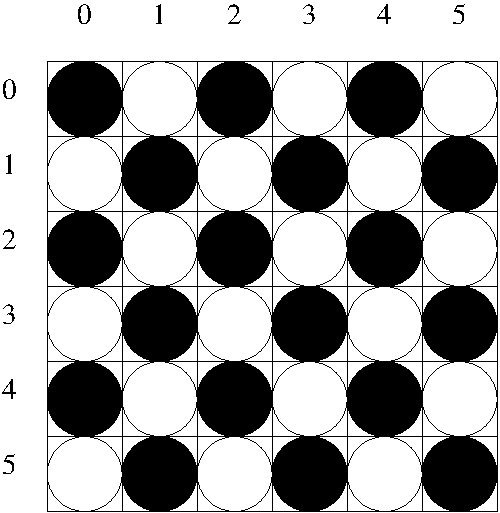
\includegraphics[width=2.5in]{images/konane1.pdf}
\end{center}
\caption{This is a caption on the figure}
\label{somefigure}
\end{figure}

\begin{table}
\begin{center}
\begin{tabular}{|c||c|cc}
\hline
& col1 & col2 & col3\\
\hline \hline
row1 & a & b & c\\
\hline 
row2 & d & e & f\\
\hline 
row3 & g &   & h\\
 & i & j & k\\
\hline 
\end{tabular}
\end{center}
\caption{This is a caption on the table.  Try to keep your captions short; don't
put multiple paragraphs of text in here.  Put the long version in the Results
section, and reference the table from there.}
\label{sometable}
\end{table}

The results section should contain your results.  It should \emph{not} contain
your interpretation of those results.  That comes later.  This section should be
made up primarily of graphs and tables that show your data.  You should also
have a small amount of text describing what each of the tables and graphs shows,
since the caption on the figures should be short.  Having text describing the
specifics of the experiment that lead to that particular table would also be
good.  For example,

\begin{quote}
``Table \ref{sometable} shows the average results of the three algorithms on all
the data sets.  The parameters used were $N=7$, and $k=3.27$; these parameters
were found by hand, and little effort was made to tune them optimally.  Each
algorithm was run three times on each of the seven data sets, and the resulting
accuracy scores were averaged.''
\end{quote}

I'm not going to tell you exactly what tables or graphs you should have here,
since it will depend a bit on your results.  You should be sure that your
results section contains sufficient data to support your conclusions about the
relative strengths and weaknesses of the different algorithms.  You should also
be sure that your data is complete; that is, don't leave data out simply because
it doesn't support the point you're trying to make.

You should also be sure that your results are clear and interpretable.  Seven
pages of raw binary data will do nothing to edify your reader.  Similarly, a
1 inch square graph with 12 lines plotted on it will be difficult to extract
meaning from, as will a graph with poor (or no) labels on the axes.  Your
results should be legible both on screen and in hard copy.

You don't want to present results that are just raw data, since that is hard to
interpret.  But you don't want to over abstract, either, since that leads to
results that have little or no meaning (eg. ``the average over all different
data sets, algorithms, and parameters'' is a completely useless statistic for
comparing algorithms).

If you are trying do draw comparisons between certain things, try to make sure
your results are presented in a way that allows the reader to easily compare
them.  This might mean having two lines in the same graph, or it might mean
having the columns you want to compare be adjacent in a table.  You want it to
be easy for the reader to follow whatever reasoning you make in your Conclusions
section by looking at your Results.  You don't want to redundancy (don't put the
same data in multiple different tables), but you want the reader to be able to
evaluate your conclusions without having to compare things that are three pages
apart in your Results.

You should probably have a page or two of results; one or two tables are unlikely to be
sufficient to describe your experiments.  If they are, you need to do more
experiments.  On the other hand, if you have more than three pages, you're
probably not doing a good job of presenting your data in a clear and concise
form.

\section{Discussion}
The discussion section is where you discuss your interpretation of the data you
presented in the results section.  This is where you tell the reader how great
your algorithm is, and how interesting it is that \emph{this} performed better
than \emph{that} on some given data set.  You can also speculate about causes
for interesting behaviors; for example, if you think you might know why it fails
so badly on some particular case, or if you have an insight into why it did well
on another case.  You don't want to be making wild guesses, but as long as you
make it clear that you are not making claims of factual proof, you can go out on
a limb a little.  For example,

\begin{quote}
``In most cases, algorithm A outperforms algorithm B with a significance of
99.8\%.  However, as can be seen from Figure \ref{somefigure}, when applied to
the ``E. E. Smith'' data set, algorithm A does no better than random chance.  It
seems likely that the failure of algorithm A to learn is due to the extremely
sparse distribution of that data set.  Because of algorithm A's heavy reliance
on data being densely sampled from the true underlying distribution, any sparse
data set is likely to show this behavior.''
\end{quote}

Think about the kinds of questions that were posed in the written portions of
homework assignments 1 and 2; these are the kinds of things you want to think
about for your Discussion.

\section{Conclusions}
The conclusion section should be relatively short, and should not be a summary
of your paper.  It should, however, bring up what you learned and what impact
your results have on the rest of the field (and society as a whole, if
applicable, but don't overstate the impact of what you're doing).  You should
conclude, and bring your paper to an end with any parting thoughts that are
appropriate.

Certain types of papers can be ended with a ``Summary'' section instead of a
``Conclusions'' section, in which case you would, in fact, summarize the main
points of your paper.  For this paper, you should write a Conclusions section,
not a Summary.

Conclusion also often contain information about what else you would like
to do.  Sometimes this is a separate subsection, or even a section, entitled
``Future Work.''  The basic idea here is to talk about what the next steps to
take would be.  This is of benefit to others who are interested in your
work and may want to help advance it.  It is also a chance for you to
acknowledge shortcomings in your work; since we never have infinite time to
prepare a paper, there are always more experiments that would have been nice to
include.  If you list them as future work, then it at least makes it clear that
you didn't do those things because you didn't have time, rather than because you
didn't realise that they were important to do.

In your paper, you should include a brief discussion of avenues for possible
future work in your Conclusions section.  It should be tied in with the rest of
your conclusion, and should not be an unrelated section tacked on the end (or
the middle).

% many different styles of bibliography are available; plain is fine for this
% assignment
\bibliographystyle{plain}

% the bibliography command should contain the name of your .bib file, minus the
% extension.
\bibliography{templateBibliography}

% because "document" is an environment, you need to have a closing tag at the
% end of your document.  Anything written after this tag will not be included in
% the generated output.
\end{document}

For example, here is some text that will never show up.
